\chapter{Alcènes et alcynes~: les additions électrophiles}\label{ch:b1:electrophilic-additions}

Agitons un alcène avec de l'eau de brome orangée~: la couleur disparaît
en quelques secondes. C'est le plus ancien test de la double liaison
carbone--carbone, et derrière lui se cache un mécanisme. Les électrons
$\pi$ de la double liaison, moins fortement retenus que les électrons
$\sigma$ et exposés au-dessus et au-dessous du plan de la molécule,
attaquent un réactif pauvre en électrons~; le cation formé capture
ensuite un \omterm{def:b1:electronic-effects:nucleophile}{nucléophile}. Ces deux mêmes étapes additionnent sur les
alcènes les halogénures d'hydrogène, l'eau et les dihalogènes,
décident quel carbone reçoit quelle partie du réactif, et fixent la
stéréochimie du produit. Ce chapitre les développe, avec la règle
qu'un chimiste du dix-neuvième siècle a tirée de
l'observation et le \omterm{def:b1:electronic-effects:intermediates}{carbocation} qui l'explique.

\begin{recall}
Les \omterm{def:b1:electronic-effects:intermediates}{carbocations}, leur stabilité et les \omterm{def:b1:electronic-effects:curly-arrow}{flèches courbes}
(\cref{ch:b1:electronic-effects})~; le postulat de Hammond
(\cref{prop:b1:elementary-steps:hammond})~; les descripteurs $Z$/$E$,
\cip{R}/\cip{S}, les \omterm{def:b1:stereochemistry-in-depth:enantiomers}{composés méso} et les \omterm{def:b1:stereochemistry-in-depth:enantiomers}{mélanges racémiques}
(\cref{ch:b1:stereochemistry-in-depth}). Le volume scolaire (année 12)
énumérait les additions sur les alcènes sans leurs mécanismes.
\end{recall}

\section{La liaison \texorpdfstring{$\pi$}{pi}, un nucléophile}

\begin{definition}[Addition électrophile]\label{def:b1:electrophilic-additions:electrophilic-addition}
Une \emph{addition électrophile}\index{addition electrophile@addition électrophile} sur une
liaison multiple est une addition dont la première étape est l'attaque
des électrons $\pi$ sur un \omterm{def:b1:electronic-effects:nucleophile}{électrophile} E~: il se forme un cation, qui
capture ensuite un \omterm{def:b1:electronic-effects:nucleophile}{nucléophile} Nu, si bien que E et Nu se retrouvent sur
les deux carbones de l'ancienne double liaison.
\end{definition}

La liaison $\pi$ est la plus faible des deux liaisons de C=C (\cref{ch:b1:lewis-resonance-vsepr}),
et ses électrons se trouvent loin des noyaux, au-dessus et au-dessous du
plan~: les alcènes sont des \omterm{def:b1:electronic-effects:nucleophile}{nucléophiles}, et réagissent avec les acides,
les dihalogènes et d'autres \omterm{def:b1:electronic-effects:nucleophile}{électrophiles} qui laissent intacts les
alcanes saturés.

\section{Halogénures d'hydrogène~: la règle de Markovnikov}

\begin{omfigure}
\setchemfig{atom sep=2.1em}
\schemestart
\chemfig{H_3C-[:30]@{c2}CH=[@{pi},,,,]@{c1}CH_2}
\+
\chemfig{@{h}H-[@{hb}]@{br}Br}
\arrow{->}
\chemfig{H_3C-[:30]CH^{+}-[:-30]CH_3}
\+
\chemfig{Br^{-}}
\arrow{->}
\chemfig{H_3C-[:30]CH(-[2]Br)-[:-30]CH_3}
\schemestop
\chemmove{\draw[->, thick, shorten <=2pt, shorten >=2pt](pi) .. controls +(90:7mm) and +(110:7mm) .. (h);
          \draw[->, thick, shorten <=2pt, shorten >=2pt](hb) .. controls +(-90:5mm) and +(-90:5mm) .. (br);}

{\small Addition du bromure d'hydrogène sur le propène. Le doublet $\pi$
capte le proton, qui se fixe sur le carbone terminal, ce qui donne le
\omterm{def:b1:electronic-effects:intermediates}{carbocation} secondaire~; l'ion bromure s'y additionne~:
2-bromopropane.}
\end{omfigure}

\begin{proposition}[Règle de Markovnikov]\label{prop:b1:electrophilic-additions:markovnikov}
Lors de l'addition de HX sur un alcène dissymétrique, l'hydrogène se
fixe sur le carbone de la double liaison qui porte déjà le plus
d'hydrogènes (\emph{règle de Markovnikov}\index{regle de Markovnikov@règle de Markovnikov}).
Sous forme moderne~: l'\omterm{def:b1:electronic-effects:nucleophile}{électrophile} s'additionne de façon à donner le
\omterm{def:b1:electronic-effects:intermediates}{carbocation} le plus stable.
\end{proposition}

\begin{proof}
Le transfert de proton est l'\omterm{def:b1:elementary-steps:rds}{étape cinétiquement déterminante}~; il est
endothermique et aboutit à un \omterm{def:b1:electronic-effects:intermediates}{carbocation}. D'après le postulat de
Hammond (\cref{prop:b1:elementary-steps:hammond}), son \omterm{def:b1:elementary-steps:energy-profile}{état de
transition} ressemble au \omterm{def:b1:electronic-effects:intermediates}{carbocation}~: la voie qui mène au \omterm{def:b1:electronic-effects:intermediates}{carbocation} le
plus stable a la barrière la plus basse et est beaucoup plus rapide.
Placer le proton sur le carbone le plus hydrogéné laisse la charge sur
le carbone qui porte le plus de groupes alkyle, le cation le plus stable
(\cref{prop:b1:electronic-effects:carbocation-order}).
\end{proof}

\begin{omfigure}
\begin{tikzpicture}
\begin{axis}[
  width=0.78\linewidth, height=5.0cm, xmin=0, xmax=10, ymin=-45, ymax=125,
  axis x line=bottom, axis y line=left, xlabel={coordonnée réactionnelle},
  ylabel={énergie}, xtick=\empty, ytick=\empty, label style={font=\small},
  legend style={font=\scriptsize, draw=none, at={(0.5,-0.30)}, anchor=north}, legend columns=2]
\addplot[omThm, thick, dashed] table[x=x, y=E] {figdata/out/bachelor-1-energy-profiles-primary.dat};
\addplot[omDef, very thick] table[x=x, y=E] {figdata/out/bachelor-1-energy-profiles-secondary.dat};
\legend{par le cation primaire, par le cation secondaire}
\node[font=\scriptsize, anchor=south] at (axis cs:5,103) {\ce{CH3CH2CH2+}};
\draw[omThm, densely dotted] (axis cs:5,103) -- (axis cs:5,87);
\node[font=\scriptsize, anchor=north] at (axis cs:5,43) {\ce{CH3CH+CH3}};
\node[font=\scriptsize, anchor=north west] at (axis cs:0.1,-3) {propène + HBr};
\end{axis}
\end{tikzpicture}

{\small \omterm{def:b1:elementary-steps:energy-profile}{Profils énergétiques} schématiques des deux additions possibles de
HBr sur le propène. Le \omterm{def:b1:electronic-effects:intermediates}{carbocation} secondaire, plus stable, est plus bas
en énergie, et, d'après le postulat de Hammond, l'\omterm{def:b1:elementary-steps:energy-profile}{état de transition} qui
y conduit l'est aussi~: le produit de Markovnikov se forme beaucoup plus
vite.}
\end{omfigure}

\begin{definition}[Réarrangement de carbocation]\label{def:b1:electrophilic-additions:rearrangement}
Un \emph{réarrangement de carbocation}\index{rearrangement de carbocation@réarrangement de carbocation}
est la migration, au sein d'un \omterm{def:b1:electronic-effects:intermediates}{carbocation}, d'un atome d'hydrogène ou
d'un groupe alkyle, avec son \omterm{def:b1:lewis-resonance-vsepr:lewis}{doublet liant}, vers le carbone cationique
voisin, ce qui donne un \omterm{def:b1:electronic-effects:intermediates}{carbocation} plus stable (une migration-1,2).
\end{definition}

\begin{example}[Une migration de méthyle]\label{ex:b1:electrophilic-additions:shift}
Le 3,3-diméthylbut-1-ène et le chlorure d'hydrogène donnent un
\omterm{def:b1:electronic-effects:intermediates}{carbocation} secondaire voisin d'un carbone quaternaire~; un groupe
méthyle migre avec son doublet et forme un cation tertiaire. Le produit
majoritaire est le 2-chloro-2,3-diméthylbutane, dont le squelette
diffère de celui de l'alcène~; le 3-chloro-2,2-diméthylbutane est
minoritaire.
\end{example}

\begin{omfigure}
\setchemfig{atom sep=2em}
\schemestart
\chemfig{C(-[2]CH_3)(-[6]CH_3)(-[4]H_3C)-CH^{+}-CH_3}
\arrow{->[migration]}[,1.5]
\chemfig{C^{+}(-[2]CH_3)(-[4]H_3C)-CH(-[6]CH_3)-CH_3}
\arrow{->[\ce{Cl-}]}
\chemfig{C(-[2]CH_3)(-[6]Cl)(-[4]H_3C)-CH(-[6]CH_3)-CH_3}
\schemestop
\par\vspace{6pt}

{\small Réarrangement du cation 3,3-diméthylbutan-2-yle~: un groupe
méthyle migre vers le carbone cationique et change le cation secondaire
en cation tertiaire, capturé par l'ion chlorure.}
\end{omfigure}

\section{L'addition de l'eau}

\begin{definition}[Hydratation d'un alcène]\label{def:b1:electrophilic-additions:hydration}
L'\emph{hydratation}\index{hydratation} d'un alcène est l'addition
d'eau, catalysée par un \omterm{def:b1:predominant-reaction:strong-acid}{acide fort}, qui donne un alcool~: l'inverse de
la \omterm{def:b1:alcohol-activation:dehydration}{déshydratation} du \cref{ch:b1:alcohol-activation}.
\end{definition}

Le mécanisme est celui de HX, l'eau jouant le rôle de \omterm{def:b1:electronic-effects:nucleophile}{nucléophile}~:
protonation (Markovnikov), capture du \omterm{def:b1:electronic-effects:intermediates}{carbocation} par l'eau, perte d'un
proton de l'ion oxonium. Le propène donne le propan-2-ol, le
2-méthylpropène le 2-méthylpropan-2-ol. \omterm{def:b1:electrophilic-additions:hydration}{Hydratation} et \omterm{def:b1:alcohol-activation:dehydration}{déshydratation}
sont un seul et même équilibre,
\ce{C3H6 + H2O <=> C3H8O}~; un acide dilué en solution aqueuse et une
basse température favorisent l'alcool, un acide concentré, le chauffage
et l'élimination de l'alcène favorisent l'alcène
(\cref{ch:b1:extent-q-and-k}).

\section{L'addition des dihalogènes~: ions halogénonium et addition anti}

\begin{definition}[Ion halogénonium, addition anti et syn]\label{def:b1:electrophilic-additions:halonium}
Lors de l'addition de \ce{Br2} ou de \ce{Cl2}, le doublet $\pi$ attaque
un atome d'halogène tandis qu'un \omterm{def:b1:lewis-resonance-vsepr:lewis}{doublet non liant} de cet atome se lie au
second carbone~: il se forme un \emph{ion halogénonium}\index{ion halogenonium@ion halogénonium}
cyclique à trois atomes, l'autre atome d'halogène partant sous forme
d'halogénure. Une addition dans laquelle les deux nouveaux groupes se
retrouvent sur des faces opposées de l'ancienne double liaison est une
\emph{addition anti}\index{addition anti}~; sur la même face, une
\emph{addition syn}\index{addition syn}.
\end{definition}

\begin{proposition}[L'addition des dihalogènes est anti]\label{prop:b1:electrophilic-additions:anti-addition}
L'addition du dibrome sur un alcène est une \omterm{def:b1:electrophilic-additions:halonium}{addition anti}~: le
\cip{E}-but-2-ène donne le méso-2,3-dibromobutane, et le
\cip{Z}-but-2-ène le \omterm{def:b1:stereochemistry-in-depth:enantiomers}{mélange racémique} de \cip{2R,3R}- et de
\cip{2S,3S}-2,3-dibromobutane.
\end{proposition}

\begin{proof}
L'ion bromonium ponte une face de l'ancienne double liaison~; l'ion
bromure ne peut attaquer un carbone que par l'autre face, ouvrant le
cycle comme une SN2, avec inversion sur ce carbone. Les deux bromes se
retrouvent sur des faces opposées. Pour le \cip{E}-but-2-ène, l'attaque
sur l'un ou l'autre carbone donne le même produit, dans lequel les deux
\omterm{def:b1:stereochemistry-in-depth:stereocentre}{centres stéréogènes} sont images l'un de l'autre dans un miroir~:
\cip{2R,3S}, méso. Pour le \cip{Z}-but-2-ène, l'attaque sur un carbone
donne \cip{2R,3R}, sur l'autre \cip{2S,3S}, avec la même probabilité~:
un \omterm{def:b1:stereochemistry-in-depth:enantiomers}{mélange racémique}. La démonstration par le dessin fait l'objet de
l'\cref{exo:b1:electrophilic-additions:10}.
\end{proof}

\begin{omfigure}
\begin{tikzpicture}[font=\small, >={Stealth}]
  % bromonium ion from (E)-but-2-ene
  \coordinate (a) at (0,0); \coordinate (b) at (1.4,0);
  \draw[thick] (a) -- (b);
  \node[circle, fill=white, inner sep=1pt] (br) at (0.7,1.0) {\ce{Br+}};
  \draw[thick] (a) -- (br.south west) (b) -- (br.south east);
  \draw[thick] (a) -- ++(-0.8,0.35) node[left] {H};
  \draw[thick] (a) -- ++(-0.6,-0.6) node[below left] {\ce{CH3}};
  \draw[thick] (b) -- ++(0.8,0.35) node[right] {\ce{CH3}};
  \draw[thick] (b) -- ++(0.6,-0.6) node[below right] {H};
  \node (bm) at (0.7,-1.6) {\ce{Br-}};
  \draw[->, thick, omThm] (bm) to[bend left=25] (0.12,-0.12);
  \node[align=center] at (0.7,-2.4) {attaque par la face opposée au pont};
  \draw[->, thick] (3.3,0) -- (4.4,0);
  \node[align=center] at (6.2,0) {\chemfig{C(-[:150]H_3C)(<[:210]H)(<:[2]Br)-C(<:[:30]H)(-[:-30]CH_3)(<[6]Br)}};
  \node at (6.2,-1.8) {produit anti~: méso-2,3-dibromobutane};
\end{tikzpicture}

{\small L'ion bromonium formé à partir du \cip{E}-but-2-ène, et son
ouverture par l'ion bromure par la face opposée (\omterm{def:b1:electrophilic-additions:halonium}{addition anti}). Le
produit possède deux \omterm{def:b1:stereochemistry-in-depth:stereocentre}{centres stéréogènes} de descripteurs opposés et,
dans une \omterm{def:b1:stereochemistry-in-depth:isomers}{conformation} convenable, un plan de symétrie interne~: c'est le
\omterm{def:b1:stereochemistry-in-depth:enantiomers}{composé méso}, \cip{2R,3S}.}
\end{omfigure}

\begin{inthelab}[L'eau de brome]
Le dibrome est un liquide dense, volatil, très toxique et corrosif. Le
test d'insaturation utilise de l'eau de brome diluée (ou une solution
commerciale d'un \omterm{def:b1:complexation:complex}{complexe} du dibrome), sous la hotte, quelques gouttes à
la fois~; la disparition de la couleur orangée signale une addition.
Dans l'eau, l'ion bromonium est aussi capturé par l'eau, et une
bromhydrine se forme à côté du dérivé dibromé.
\end{inthelab}

\section{Les alcynes~: additions et acétylures}

Les alcynes additionnent HX et \ce{X2} deux fois, chaque étape se
déroulant comme pour les alcènes (Markovnikov pour HX). Leur \omterm{def:b1:electrophilic-additions:hydration}{hydratation},
catalysée par un acide et un sel de mercure(II), ne donne pas l'alcool
insaturé attendu mais une cétone~: un énol se réarrange aussitôt en
composé carbonylé, processus étudié dans le volume de deuxième année.

\begin{definition}[Alcyne terminal, acétylure]\label{def:b1:electrophilic-additions:acetylide}
Un \emph{alcyne terminal}\index{alcyne terminal} \ce{R-C#C-H} a sa
triple liaison en bout de chaîne. Une \omterm{def:b1:predominant-reaction:strong-acid}{base forte} (l'amidure de sodium)
arrache son hydrogène, ce qui donne l'\emph{ion acétylure}\index{ion acetylure@ion acétylure}
\ce{R-C#C-}, un bon \omterm{def:b1:electronic-effects:nucleophile}{nucléophile} carboné.
\end{definition}

\begin{proposition}[Acidité des alcynes terminaux]\label{prop:b1:electrophilic-additions:acetylide-acidity}
La liaison C--H d'un \omterm{def:b1:electrophilic-additions:acetylide}{alcyne terminal} est bien plus acide que celles des
alcènes et des alcanes, tout en restant beaucoup moins acide que l'eau~:
les acétylures se forment avec les ions amidure, non avec l'hydroxyde,
et sont détruits par l'eau.
\end{proposition}

\begin{proof}
Dans l'\omterm{def:b1:electrophilic-additions:acetylide}{ion acétylure}, le \omterm{def:b1:lewis-resonance-vsepr:lewis}{doublet non liant} occupe une orbitale à moitié
de caractère \textit{s} (carbone \textit{sp}), plus proche du noyau que
les orbitales des \omterm{def:b1:electronic-effects:intermediates}{carbanions} \textit{sp}$^2$ ou \textit{sp}$^3$~: il est
plus stable, et son acide conjugué plus fort. Il reste une base bien plus
forte que l'hydroxyde, si bien que l'eau le protone.
\end{proof}

Un acétylure attaque un halogénoalcane primaire par SN2 (nouvelle
liaison C--C, \ce{R-C#C-} + $\mathrm{R'Br}$) ou s'additionne sur un
carbonyle comme un \omterm{def:b1:organomagnesium:organometallic}{organomagnésien}~: une autre façon de construire des
squelettes carbonés.

\begin{method}[Prévoir une addition]\label{met:b1:electrophilic-additions:predict-addition}
\begin{enumerate}
  \item Repérer l'\omterm{def:b1:electronic-effects:nucleophile}{électrophile} (\ce{H+}, \ce{Br2}) et le \omterm{def:b1:electronic-effects:nucleophile}{nucléophile} qui
        suivra (\ce{X-}, l'eau, l'halogénure).
  \item Pour \ce{H+}~: le fixer sur le carbone qui donne le \omterm{def:b1:electronic-effects:intermediates}{carbocation}
        le plus stable (Markovnikov)~; envisager une éventuelle
        migration-1,2.
  \item Pour \ce{X2}~: former l'\omterm{def:b1:electrophilic-additions:halonium}{ion halogénonium} ponté et l'ouvrir par
        la face opposée (anti)~; dessiner les deux attaques possibles et
        comparer les produits (méso ou racémique).
  \item En présence d'eau, attendre aussi l'alcool (ou l'halohydrine).
\end{enumerate}
\end{method}

\begin{history}[Vladimir Markovnikov]
\begin{minipage}[t]{0.2\linewidth}\vspace{0pt}
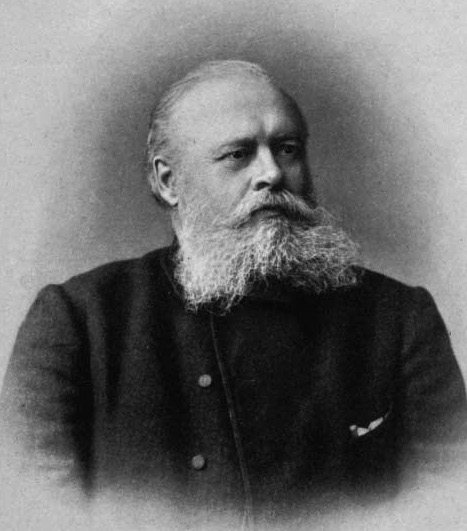
\includegraphics[width=\linewidth]{images/book2/markovnikov.jpg}
\end{minipage}\hfill
\begin{minipage}[t]{0.76\linewidth}\vspace{0pt}
Vladimir Markovnikov a énoncé sa règle au dix-neuvième siècle,
à partir des produits que lui et d'autres observaient, bien avant que
n'existent les \omterm{def:b1:electronic-effects:intermediates}{carbocations} ou les \omterm{def:b1:electronic-effects:curly-arrow}{flèches courbes}~: une régularité de
la nature, consignée avant de pouvoir être expliquée. Son énoncé moderne
fondé sur la stabilité des \omterm{def:b1:electronic-effects:intermediates}{carbocations} montre ce qu'un mécanisme ajoute
à une règle empirique~: il dit quand la règle doit échouer. (Portrait
tiré d'une notice nécrologique publiée en 1905, domaine public,
Wikimedia Commons.)
\end{minipage}
\end{history}

\section{Exercices}

\begin{exercise}[$\star$]\label{exo:b1:electrophilic-additions:1}
Donner le produit majoritaire de~: propène + HCl~; 2-méthylpropène +
HBr~;
1-méthylcyclohexène + HBr~; but-2-yne + un équivalent de HCl.
\end{exercise}

\begin{exercise}[$\star$]\label{exo:b1:electrophilic-additions:2}
Écrire les produits du dibrome avec l'éthène, le cyclohexène et le
propène. Les nommer.
\end{exercise}

\begin{exercise}[$\star$]\label{exo:b1:electrophilic-additions:3}
Quel alcool l'\omterm{def:b1:electrophilic-additions:hydration}{hydratation} acido-catalysée de chacun de ces alcènes
donne-t-elle~: propène, 2-méthylpropène, méthylènecyclohexane~?
\end{exercise}

\begin{exercise}[$\star$]\label{exo:b1:electrophilic-additions:4}
Lesquels de ces composés réagissent avec l'amidure de sodium~: propyne,
but-2-yne, propène, éthanol~? Écrire les réactions.
\end{exercise}

\begin{exercise}[$\star\star$]\label{exo:b1:electrophilic-additions:5}
Écrire le mécanisme complet de l'\omterm{def:b1:electrophilic-additions:hydration}{hydratation} du 2-méthylpropène avec des
\omterm{def:b1:electronic-effects:curly-arrow}{flèches courbes}, et expliquer pourquoi la réaction inverse est favorisée
dans l'acide concentré chaud.
\end{exercise}

\begin{exercise}[$\star\star$]\label{exo:b1:electrophilic-additions:6}
Expliquer à l'aide du postulat de Hammond pourquoi le 2-méthylpropène
réagit avec HCl beaucoup plus vite que le propène.
\end{exercise}

\begin{exercise}[$\star\star$]\label{exo:b1:electrophilic-additions:7}
Le dibrome réagit avec le cyclohexène. Montrer que le produit est le
\textit{trans}-1,2-dibromocyclohexane, et dire s'il est \omterm{def:b1:stereochemistry-in-depth:stereocentre}{chiral} et si le
produit obtenu est optiquement actif.
\end{exercise}

\begin{exercise}[$\star\star$]\label{exo:b1:electrophilic-additions:8}
Proposer un mécanisme pour l'addition de HCl sur le 3-méthylbut-1-ène
qui donne surtout le 2-chloro-2-méthylbutane.
\end{exercise}

\begin{exercise}[$\star\star$]\label{exo:b1:electrophilic-additions:9}
Proposer une synthèse de l'hex-2-yne à partir du propyne et d'un
halogénoalcane, et du 1-phénylbut-2-yn-1-ol à partir du propyne et du
benzaldéhyde.
\end{exercise}

\begin{exercise}[$\star\star\star$]\label{exo:b1:electrophilic-additions:10}
Démontrer par le dessin la stéréochimie de l'addition du dibrome sur les
deux but-2-ènes~: ion bromonium, attaque anti sur chaque carbone,
\omterm{def:b1:stereochemistry-in-depth:representations}{représentation de Cram} des produits, descripteurs. Dénombrer les
\omterm{def:b1:stereochemistry-in-depth:isomers}{stéréoisomères} formés dans chaque cas.
\end{exercise}

\begin{exercise}[$\star\star\star$]\label{exo:b1:electrophilic-additions:11}
L'eau de brome donne avec le propène le 1-bromopropan-2-ol comme produit
majoritaire. Expliquer la régiosélectivité~: pourquoi l'eau attaque-t-elle
le carbone le plus substitué de l'ion bromonium~?
\end{exercise}

\begin{exercise}[$\star\star\star$]\label{exo:b1:electrophilic-additions:12}
Un hydrocarbure \ce{C5H10} décolore l'eau de brome et additionne HBr en
donnant le 2-bromo-2-méthylbutane~; son \omterm{def:b1:electrophilic-additions:hydration}{hydratation} donne le
2-méthylbutan-2-ol. Trouver deux structures possibles et proposer un
moyen de les distinguer.
\end{exercise}

\section{Problème~: deux butènes et le dibrome}

\begin{problem}[{Problème du week-end --- les deux but-2-ènes, le
mécanisme par l'ion bromonium, les dérivés dibromés méso et racémique,
leur pouvoir rotatoire et la masse obtenue}]
\label{pb:b1:electrophilic-additions:1}
Un laboratoire dispose de deux flacons de but-2-ène, l'un de \cip{Z} pur,
l'autre d'\cip{E} pur, et traite \qty{5.60}{g} de chacun par le dibrome
dans le dichlorométhane. Masses molaires (\unit{g/mol})~: \ce{C4H8} 56.0, \ce{Br2}
159.8, \ce{C4H8Br2} 215.8.

\medskip
\noindent\textbf{Partie I --- Les deux alcènes.}
\begin{enumerate}
  \item Dessiner le \cip{Z}- et l'\cip{E}-but-2-ène et justifier les
        descripteurs.
  \item Sont-ils des \omterm{def:b1:stereochemistry-in-depth:isomers}{stéréoisomères}~? Des \omterm{def:b1:stereochemistry-in-depth:enantiomers}{énantiomères} ou des
        \omterm{def:b1:stereochemistry-in-depth:enantiomers}{diastéréoisomères}~?
  \item Pourquoi ne s'interconvertissent-ils pas à température ambiante~?
  \item Lequel est le plus stable, et pourquoi~?
  \item Écrire l'équation globale de l'addition du dibrome.
  \item Combien de \omterm{def:b1:stereochemistry-in-depth:stereocentre}{centres stéréogènes} le 2,3-dibromobutane
        possède-t-il~? Combien de \omterm{def:b1:stereochemistry-in-depth:isomers}{stéréoisomères} au plus, et combien en
        réalité~?
\end{enumerate}

\medskip
\noindent\textbf{Partie II --- Le mécanisme.}
\begin{enumerate}[resume]
  \item Écrire la formation de l'ion bromonium avec des \omterm{def:b1:electronic-effects:curly-arrow}{flèches courbes}.
  \item Pourquoi se forme-t-il un ion bromonium ponté plutôt qu'un
        \omterm{def:b1:electronic-effects:intermediates}{carbocation} ouvert~?
  \item Écrire l'ouverture de l'ion par l'ion bromure.
  \item Pourquoi l'ion bromure attaque-t-il par la face opposée au pont~?
  \item Quel type d'addition en résulte-t-il~?
  \item Pourquoi le solvant est-il le dichlorométhane et non l'eau~?
\end{enumerate}

\medskip
\noindent\textbf{Partie III --- Les produits.}
\begin{enumerate}[resume]
  \item À partir du \cip{E}-but-2-ène~: dessiner le produit de l'attaque
        sur C2 et donner les descripteurs de C2 et C3.
  \item Même question pour l'attaque sur C3. Comparer.
  \item Montrer que le produit est méso.
  \item À partir du \cip{Z}-but-2-ène~: dessiner les deux produits et
        leurs descripteurs.
  \item Dans quelles proportions se forment-ils~? Nommer le mélange.
  \item La réaction est-elle stéréospécifique~? Justifier.
\end{enumerate}

\medskip
\noindent\textbf{Partie IV --- Pouvoir rotatoire et masse.}
\begin{enumerate}[resume]
  \item Quel pouvoir rotatoire le produit issu de l'alcène \cip{Z}
        présente-t-il~?
  \item Calculer la quantité de matière de chaque alcène.
  \item Calculer la masse de dérivé dibromé attendue à partir de chacun
        pour un \omterm{def:b1:extent-q-and-k:fractional-extent}{rendement} de \qty{85}{\percent}.
  \item Donner le \omterm{def:b1:stereochemistry-in-depth:optical-activity}{pouvoir rotatoire spécifique} du dérivé dibromé obtenu à
        partir de l'\cip{E}-but-2-ène, et la masse obtenue.
\end{enumerate}
\end{problem}
